\chapter{Análisis y diseño}

En este capítulo se describe el análisis y el diseño del trabajo propuesto para
la recolección, clasificación de noticias y el entorno web.

%------------------------Requisitos Funcionales ------------------%
\section{Requisitos funcionales}

%----------------------------RF1------------------------------%
   \Dline{RF1}{Recolectar noticias}
    \begin{itemize}
      \item \textbf{Descripción:} El sistema debe recolectar noticias de forma automática en Internet.\\
    \end{itemize}
%----------------------------RF2------------------------------%
   \Dline{RF2}{Clasificar noticias}
    \begin{itemize}
      \item \textbf{Descripción:} El sistema debe clasificar las noticias recolectadas de acuerdo a su contenido.\\
    \end{itemize}
%----------------------------RF3------------------------------%
   \Dline{RF3}{Mostrar resultados}
    \begin{itemize}
      \item \textbf{Descripción:} El sistema mostrará las URLs de las noticias que cumplan con los criterios de búsqueda establecidos.\\
    \end{itemize}


%------------------------Requisitos No Funcionales ---------------%
\section{Requisitos no funcionales}



%----------------------------RNF1------------------------------%
   \DVline{RNF1}{Tiempo de clasificación}
    \begin{itemize}
      \item \textbf{Descripción:} La clasificación de una noticia no debe tardar mas de cinco segundo.\\
    \end{itemize}

%----------------------------RNF2------------------------------%
   \DVline{RNF2}{Número de palabras}
    \begin{itemize}
     \item \textbf{Descripción:} Las noticias recolectads deberán tener un mínimo de 180 palabras en ellas.\\
    \end{itemize}

%----------------------------RNF3------------------------------%  
   \DVline{RNF3}{Número de noticias mostradas}
    \begin{itemize}
      \item \textbf{Descripción:} En el sitio web, se den visualizar almenos 15 noticias.\\
    \end{itemize}

%----------------------------RNF4------------------------------%  
   \DVline{RNF4}{Tiempo de actualización}
    \begin{itemize}
      \item \textbf{Descripción:} El tiempo para mostrar las 15 noticias clasificadas no debe exceder los 3 segundos.\\
    \end{itemize}


%----------------------------Reglas de negocio---------------------%  
\section{Reglas de negocio}


En esta sección se describen las reglas de negocio implementadas en el trabajo propuesto.\\\\
%------------------RN1-----------------------%
\DGline{RN1}{Número de palabras}
\begin{itemize}
  \item \textbf{Tipo:}  
  \item \textbf{Descripción:}  La notica debe tener almenos 180 palabras
  \item \textbf{Ejemplo:}
  \item \textbf{Refer:}
\end{itemize}
%------------------RN2-----------------------%
\DGline{RN2}{Lenguaje de direcciones web}

\begin{itemize}
  \item \textbf{Tipo:}  
  \item \textbf{Descripción:} Las direcciones de los sitios a consultar deben estar redactadas en lenguaje español.
  \item \textbf{Referenciado por:} \Tref{CU1}{CU1 Seleccionar sección} \\
\end{itemize}
%------------------RN3-----------------------%
\DGline{RN3}{Lenguaje de noticias}

\begin{itemize}
  \item \textbf{Tipo:}  
  \item \textbf{Descripción:} Las noticias deben estar redactadas en lenguaje español mexicano.
  \item \textbf{Ejemplo:}
  \item \textbf{Referenciado por:}  \\
\end{itemize}
%------------------RN4-----------------------%
\DGline{RN4}{Restricción en la recoleción}

\begin{itemize}
  \item \textbf{Tipo:}  
  \item \textbf{Descripción:} Solo se puede recoletar información de los sitios que lo permitan.
  \item \textbf{Ejemplo:}
  \item \textbf{Referenciado por:}  \\
\end{itemize}
%------------------RN5-----------------------%
\DGline{RN5}{Porcentaje de aceptación}

\begin{itemize}
  \item \textbf{Tipo:}  
  \item \textbf{Descripción:} Solo se puede mostrar una noticia si cumple con un porcentaje de aceptación mayor a 60\%.
  \item \textbf{Ejemplo:}
  \item \textbf{Referenciado por:}  \\
\end{itemize}
%------------------RN6-----------------------%
\DGline{RN6}{Formato de fecha}

\begin{itemize}
  \item \textbf{Tipo:} Derivación.
  \item \textbf{Descripción:} El formato de fecha se define como:\\

  $F=D/M/A$

  $donde$\\ 

  $D=\{x/x\ E\ N,1\leq\ x\ \leq31\}$\\
  $M=\{y/y\ E\ N,1\leq\ y\ \leq12\}$\\
  $A=\{z/z\ E\ N,1990\leq\ z\ \leq\Lambda_i\}$\\

  $F:Fecha$\\
  $\Lambda_i:Anio\_actual$\\

  \item \textbf{Ejemplo:} 
  \item \textbf{Referenciado por:} \Tref{CU2}{CU2 Buscar noticias} \\
\end{itemize}

%------------------RN7-----------------------%
\DGline{RN7}{Perido preestablecido}

\begin{itemize}
  \item \textbf{Tipo:} Cálculo
  \item \textbf{Descripción:} El formato de fecha es el descrito en la \RNref{RN6}{Formato de fecha}; El periodo preestablecido se define de la siguiente forma.\\\\
  \textbf{Fecha fin}:Toma el valor de la fecha actual.\\
  \textbf{Fecha inicio}: Es colocada 5 día antes de la fecha actual; Se muestra la forma completa para el cálculo del día, mes y año:\\
  $Sea$\\
  $D_a:Dia\_actual$\\
  $M_a:Mes\_actual$\\
  $A_a:Anio\_actual$\\
  $F_i:Fecha\_inicio$\\
  $mod:Operacion\ modulo$\\
  $\Psi(M_a):Funcion\ dias\ de \ mes$\\

  $\xi=\frac{D_a-5}{\mid D_a-5 \mid}$\\

  $\delta=\frac{\xi(\mid\xi-1\mid)}{2}$\\

  La fecha toma el sigueinte valor:\\
  $F_i=D_c/M_c/A_c$\\ 
  Existen 4 casos para calcular el día, mes y años; Dependen del mes y el día actual: \\

  \begin{tabular}{|l|c|c|}
  	\hline
	\multicolumn{1}{| >{\columncolor{black}}l|}{ \textcolor{myWhite}{\textbf{Caso:}} }&
	\multicolumn{1}{| >{\columncolor{black}}c|}{ \textcolor{myWhite}{1} }&\multicolumn{1}{| >{\columncolor{black}}c|}{ \textcolor{myWhite}{2} }\\
	\hline
	\textbf{Restricción:}&$2\leq\ M_a\leq\ 12;D_a\neq5$  &$2\leq\ M_a\leq\ 12;D_a=5$\\
	\hline 
	\textbf{$D_c:$}&$(D_a-5)\pmod{\Psi(M_a-1)+1}$   &$\Psi(M_a-1)$\\
	\hline
	\textbf{$M_c:$}&$M_a+\delta$        			 &$M_a-1$\\
	\hline
	\textbf{$A_c:$}&$A_a$        				     &$A_a$\\
	\hline
  \end{tabular}


  \begin{tabular}{|l|c|c|}
  	\hline
	\multicolumn{1}{| >{\columncolor{black}}l|}{ \textcolor{myWhite}{\textbf{Caso:}} }&
	\multicolumn{1}{| >{\columncolor{black}}c|}{ \textcolor{myWhite}{3} }&\multicolumn{1}{| >{\columncolor{black}}c|}{ \textcolor{myWhite}{4} }\\
	\hline
	\textbf{Restricción:}&$M_a=1;D_a \neq 5$&\ \ \ \ \ \ $M_a=1;D_a=5$\ \ \ \ \ \\
	\hline 
	\textbf{$D_c:$}&\ \ \ \ \ \ \ \ \ $(D_a-5)\pmod{32}$\ \ \ \ \ \ \ \ & $31$\\
	\hline
	\textbf{$M_c:$}&$\xi\pmod{13}$&$12$\\
	\hline
	\textbf{$A_c:$}&$A_a+\delta$&$A_a-1$\\
	\hline
  \end{tabular}


  \item \textbf{Ejemplo:} 
  \item \textbf{Referenciado por:} \Tref{CU1}{CU1 Seleccionar sección}, \Tref{CU2}{CU2 Buscar noticias} \\
\end{itemize}%------------------RN8-----------------------%
\DGline{RN8}{Periodo válido}

\begin{itemize}
  \item \textbf{Tipo:} Derivación.
  \item \textbf{Descripción:}\\
  $Sea$\\

  $F_i:Fecha\_inicio$\\
  $F_f:Fecha\_fin$\\

  $T=\{Valido,Invalido\}$\\
  $\psi\ \epsilon\ T$\\

  Un periodo de fecha se defino como:\\

  $(\psi=Valido)\leftrightarrow(F_i\ \leq\ F_f)$\\
  $(\psi=Invalido)\leftrightarrow(F_i\ >\ F_f)$\\
  \item \textbf{Ejemplo:}
  \item \textbf{Referenciado por:} \Tref{CU2}{CU2 Buscar noticias} \\
\end{itemize}
%------------------RN9-----------------------%
\DGline{RN9}{Límite de periodo}

\begin{itemize}
  \item \textbf{Tipo:} Derivación. 
  \item \textbf{Descripción:} 

  $Sea$\\

  $F_i:Fecha\_inicio$\\
  $F_f:Fecha\_fin$\\
  $F_a:Fecha\_actual$\\
  $F_c:01/01/1990$\\

  $T=\{Valido,Invalido\}$\\
  $\psi\ \epsilon\ T$\\

  $\Phi=[F_c,F_a]$\\
  $I=[F_i,F_f]$\\
  

  Un intervalo de tiempo dentro de los limites del sistema se define como:\\

  $(\psi=Valido)\leftrightarrow(I\ \subseteq\ \Phi)$\\
  $(\psi=Invalido)\leftrightarrow(I\ \nsubseteq \Phi)$\\

  \item \textbf{Referenciado por:} \Tref{CU2}{CU2 Buscar noticias} \\
\end{itemize}

%------------------RN10-----------------------%
\DGline{RN10}{Campos obligatorios}

\begin{itemize}
  \item \textbf{Tipo:} Restricción.  
  \item \textbf{Descripción:} Los campos marcados con \* no se deben omitir.
  \item \textbf{Ejemplo:} 
  \item \textbf{Referenciado por:}  \\
\end{itemize}
%------------------RN11-----------------------%
\DGline{RN11}{Sitios restringidos}

\begin{itemize}
  \item \textbf{Tipo:}m
  \item \textbf{Descripción:} No se debe acceder a las siguientes páginas:
    \begin{itemize}
        \item Facebook
        \item Youtube
        \item Twitter
        \item Instagram 
    \end{itemize} 
  \item \textbf{Ejemplo:}
  \item \textbf{Referenciado por:} \Tref{CU3}{CU3 Recolectar noticias} \\
\end{itemize}
%------------------RN12-----------------------%
\DGline{RN12}{Orden de publicación}

\begin{itemize}
  \item \textbf{Tipo:} Descripción
  \item \textbf{Descripción:} Las noticias se muestrán de forma descendente deacuerdo a su fecha de difusión; Es decir la primera publicación en mostrarse es aquella que tiene la fecha y hora mas sercana a la del sistema.
  \item \textbf{Ejemplo:} 
  \item \textbf{Referenciado por:} \Tref{CU2}{CU2 Buscar noticias} \\
\end{itemize}

%------------------RN13-----------------------%
\DGline{RN13}{Profundidad de búsqueda}

\begin{itemize}
  \item \textbf{Tipo:} Cálculo.
  \item \textbf{Descripción:} Se muestra la forma correcta de realizar el cáculo para obtener la profundidad de búsqueda dependiendo del número de noticias a recolectar y la cantidad de hiperbínculos de la página.\\
 
  $Sea$\\

  $\Lambda(\psi,\mu)=\frac{\psi(\psi\mu-1)}{\psi-1}$\\\\
  $donde$\\
  $\psi:Numero\ de\ URL\ por\ pagina$\\
  $\mu:Profundidad\ de\ busqueda$\\
  $\Lambda:Numero\ de\ noticias\ recolectadas$\\

  $Corolario$\\ 
 El cálculo de la profundidad deacuerdo a $\psi$ y a un $\Lambda$ deseado se realiza de la siguiente forma:\\

  $\mu=\log_{\psi}{(\Lambda(\psi-1)+\psi)}-1$\\

  \item \textbf{Ejemplo:} 
  \item \textbf{Referenciado por:} \Tref{CU3}{CU3 Recolectar noticias}\\
\end{itemize}

%------------------RN14-----------------------%
\DGline{RN14}{Número de peticiones}

\begin{itemize}
  \item \textbf{Tipo:} Restricción
  \item \textbf{Descripción:} El número de peticiones realizadas a una página no debe exceder el permitido por el dominio.
  \item \textbf{Ejemplo:} 
  \item \textbf{Referenciado por:} \Tref{CU3}{CU3 Recolectar noticias} \\
\end{itemize}



%--------------------------Casos de uso -------------------------%

\newpage
\section{Casos de uso}

%--------------------------Diagrama CU -------------------------%
\Tsubsection{Diagrama de casos de uso}



La figura \textbf{\ref{fig:DCU}} muestra el diagrama de casos de uso de la aplicación. Los casos de uso marcados en color gris son descritos en el documento, sin embargo los mostrados en color rojo serán desarrollados posteriormente.

%\begin{figure}[h]
%  \centering
%  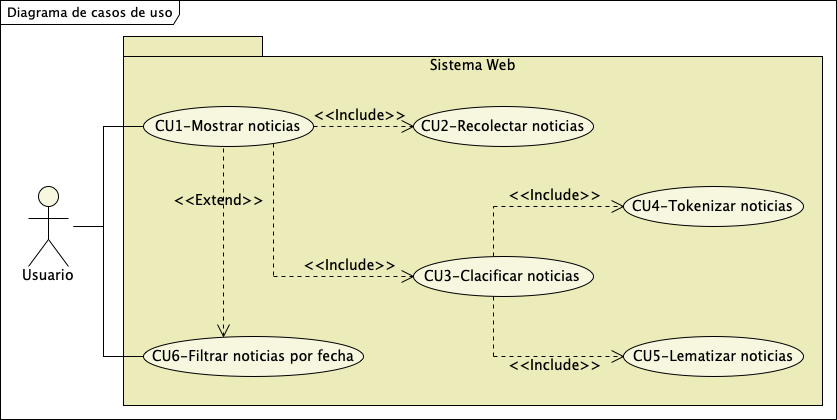
\includegraphics[scale=.4]{imagenes/Diagramas/CasosDeuso/CasosDeuso}
%  \caption{Diagrama de casos de uso}
%  \label{fig:DCU}
%\end{figure}


{\setlength{\parindent}{0pt}%Con este comando eliminos la indexación de cada párrafo%
  
  \newpage
  \input{Capitulos/Capitulo4-AnalisisYdisenio/CasosDeUso/cu1-mostrarNoticia}
  \newpage
  \input{Capitulos/Capitulo4-AnalisisYdisenio/CasosDeUso/cu2-recolectarNoticias}
  \newpage
  \input{Capitulos/Capitulo4-AnalisisYdisenio/CasosDeUso/cu3-clasificarNoticia}
  \newpage
  \input{Capitulos/Capitulo4-AnalisisYdisenio/CasosDeUso/cu4-tokenizarNoticias}
  \newpage
  \Tsubsection{CU5 Lematizar noticias}

\begin{large}
	\textbf{Resumen}\\
\end{large}

Texto.\\

\begin{large}
	\textbf{Descripción}\\
\end{large}

\begin{tabular}{|l|l|}
	\hline
	\multicolumn{1}{| >{\columncolor{black}}l|}{ \textcolor{myWhite}{\textbf{Caso de uso: }} }&
	\multicolumn{1}{| >{\columncolor{black}}l|}{ \textcolor{myWhite}{CU-1 Recolectar noticias} }\\
	\hline
	\textbf{Actor:} & 	Lorem Ipsum	\\
	\hline
	\textbf{Propósito:} & Lorem Ipsum \\
	\hline
	\textbf{Entradas:} & Lorem Ipsum \\
	\hline
	\textbf{Salidas:} & Lorem Ipsum\\
	\hline
	\textbf{Precondición:} & Lorem Ipsum \\
	\hline
	\textbf{Postcondiciones:} & Lorem Ipsum \\
	\hline
	\textbf{Reglas de negocio:} & Lorem Ipsum \\
	\hline
	\textbf{Errores:} & Lorem Ipsum \\
	\hline
	\textbf{Autor:} & Lorem Ipsum \\
	\hline
\end{tabular}\\\\

%--------------------Trayectoria Principal-----------%


\begin{large}
	\textbf{Trayectoria principal}\\
\end{large}	

\begin{enumerate}[1.]
	\item \actor lorem ipsum
	\item \sistema lorem ipsum
	\item \sistema lorem ipsum
	\item \sistema lorem ipsum
	\item \finCU	
\end{enumerate}


%--------------------trayectoria Alternatia A---------%

\begin{large}
	\textbf{Trayectoria alternativa A:}\\
\end{large}	
\textbf{Condición:} \textit{Se escribe la condición}
\begin{enumerate}[{A-}1.]

	\item \actor lorem ipsum
	\item \sistema lorem ipsum
	\item \finTA	

\end{enumerate}


%--------------------trayectoria Alternatia b---------%
\begin{large}
	\textbf{Trayectoria alternativa B:}\\
\end{large}	
\textbf{Condición:} \textit{Se escribe la condición}

\begin{enumerate}[{B-}1.]

	\item \actor lorem ipsum
	\item \sistema lorem ipsum
	\item \finTA	

\end{enumerate}


%--------------------Puntos de extención--------------------%

\begin{large}
	\textbf{Puntos de extensión}\\
\end{large}	

\textbf{Causa de la extensión:} Lorem ipsum\\
\textbf{Región de la trayectorioa:} Lorem ipsum\\
\textbf{Extiende a :} Lorem ipsum\\\\

\textbf{Causa de la extensión:} Lorem ipsum\\
\textbf{Región de la trayectorioa:} Lorem ipsum\\
\textbf{Extiende a :} Lorem ipsum\\


  \newpage
  \input{Capitulos/Capitulo4-AnalisisYdisenio/CasosDeUso/cu6-FiltrarNoticiaFecha}
  \newpage
}
  %--------------------------Descripción de pantallas ------------------%
\section{Pantallas}

\input{Capitulos/Capitulo4-AnalisisYdisenio/DescripcionPantallas/ui1-inicio}
\newpage
\subsection{UI2-Sección deportes}

\Large{\textbf{Objetivo}}\\\\
\normalsize{Texto}\\



\Large{\textbf{Descripción}}\\
\normalsize{Texto}\\


\Large{\textbf{Comandos}}\\
\normalsize{}

\begin{itemize}
	\item Lorem ipsum
	\item Lorem ipsum
	\item Lorem ipsum
\end{itemize}

\Large{\textbf{Referencia}}\\\\
\normalsize{Nombre Caso de uso}

\begin{figure}
  \centering
	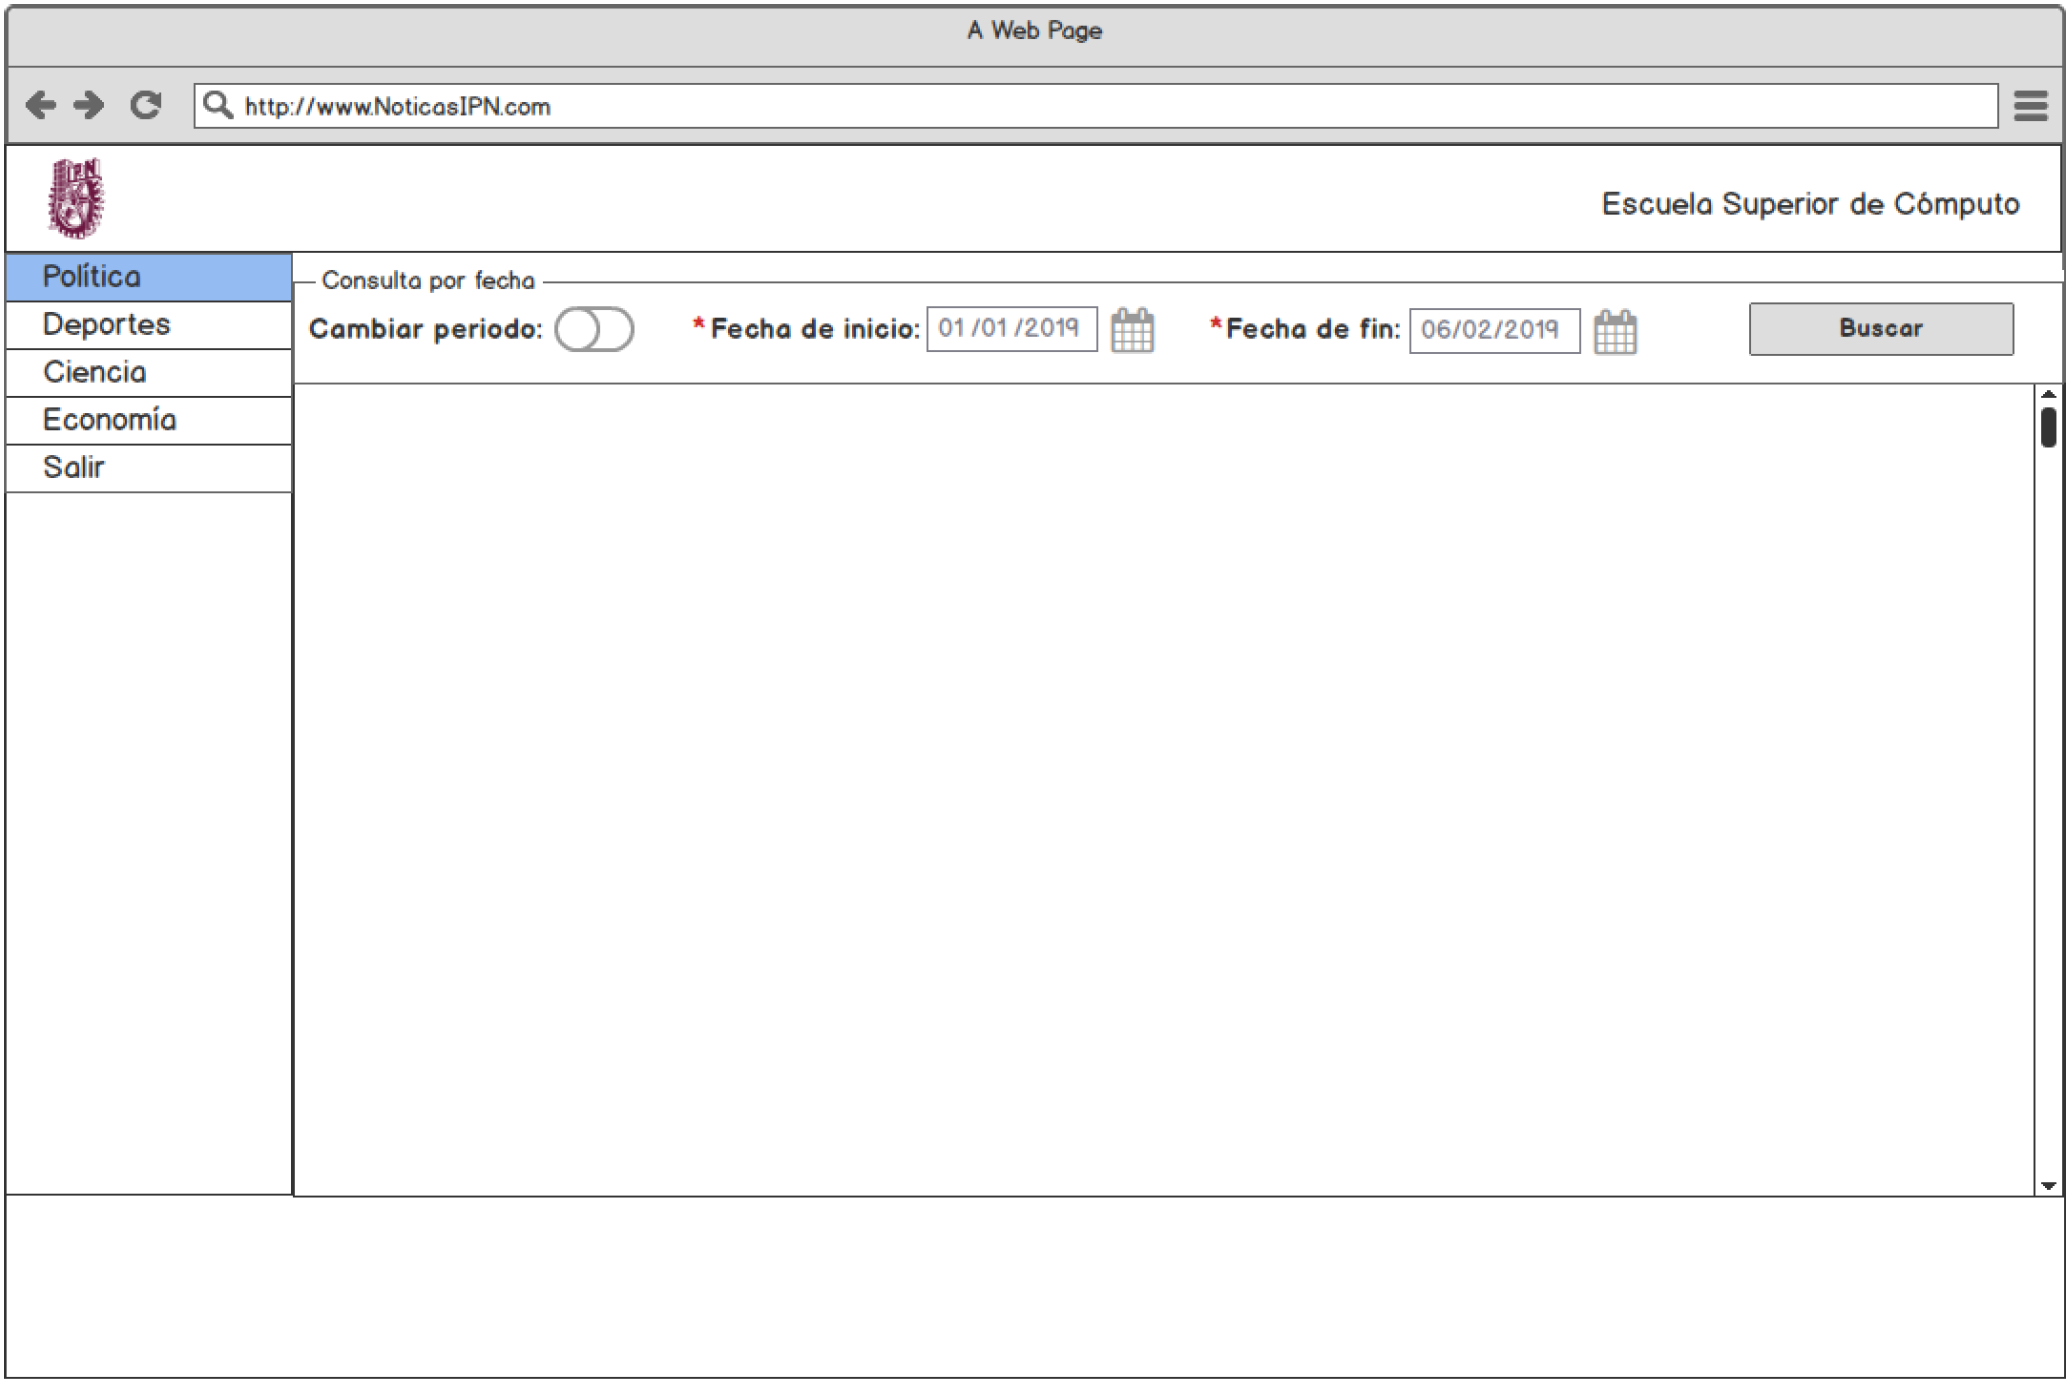
\includegraphics[scale=.3]{imagenes/Pantallas/UI2}
  \caption{Pantalla IU2-Sección deportes}
  \label{fig:IU2}
\end{figure}
\newpage
\subsection{UI3-Busqueda por fecha}

\Large{\textbf{Objetivo}}\\\\
\normalsize{Texto}\\

	

\Large{\textbf{Descripción}}\\
\normalsize{Texto}\\



\Large{\textbf{Comandos}}\\
\normalsize{}

\begin{itemize}
	\item Lorem ipsum
	\item Lorem ipsum
	\item Lorem ipsum
\end{itemize}

\Large{\textbf{Referencia}}\\\\
\normalsize{Nombre Caso de uso}

\begin{figure}[h]
  \centering
	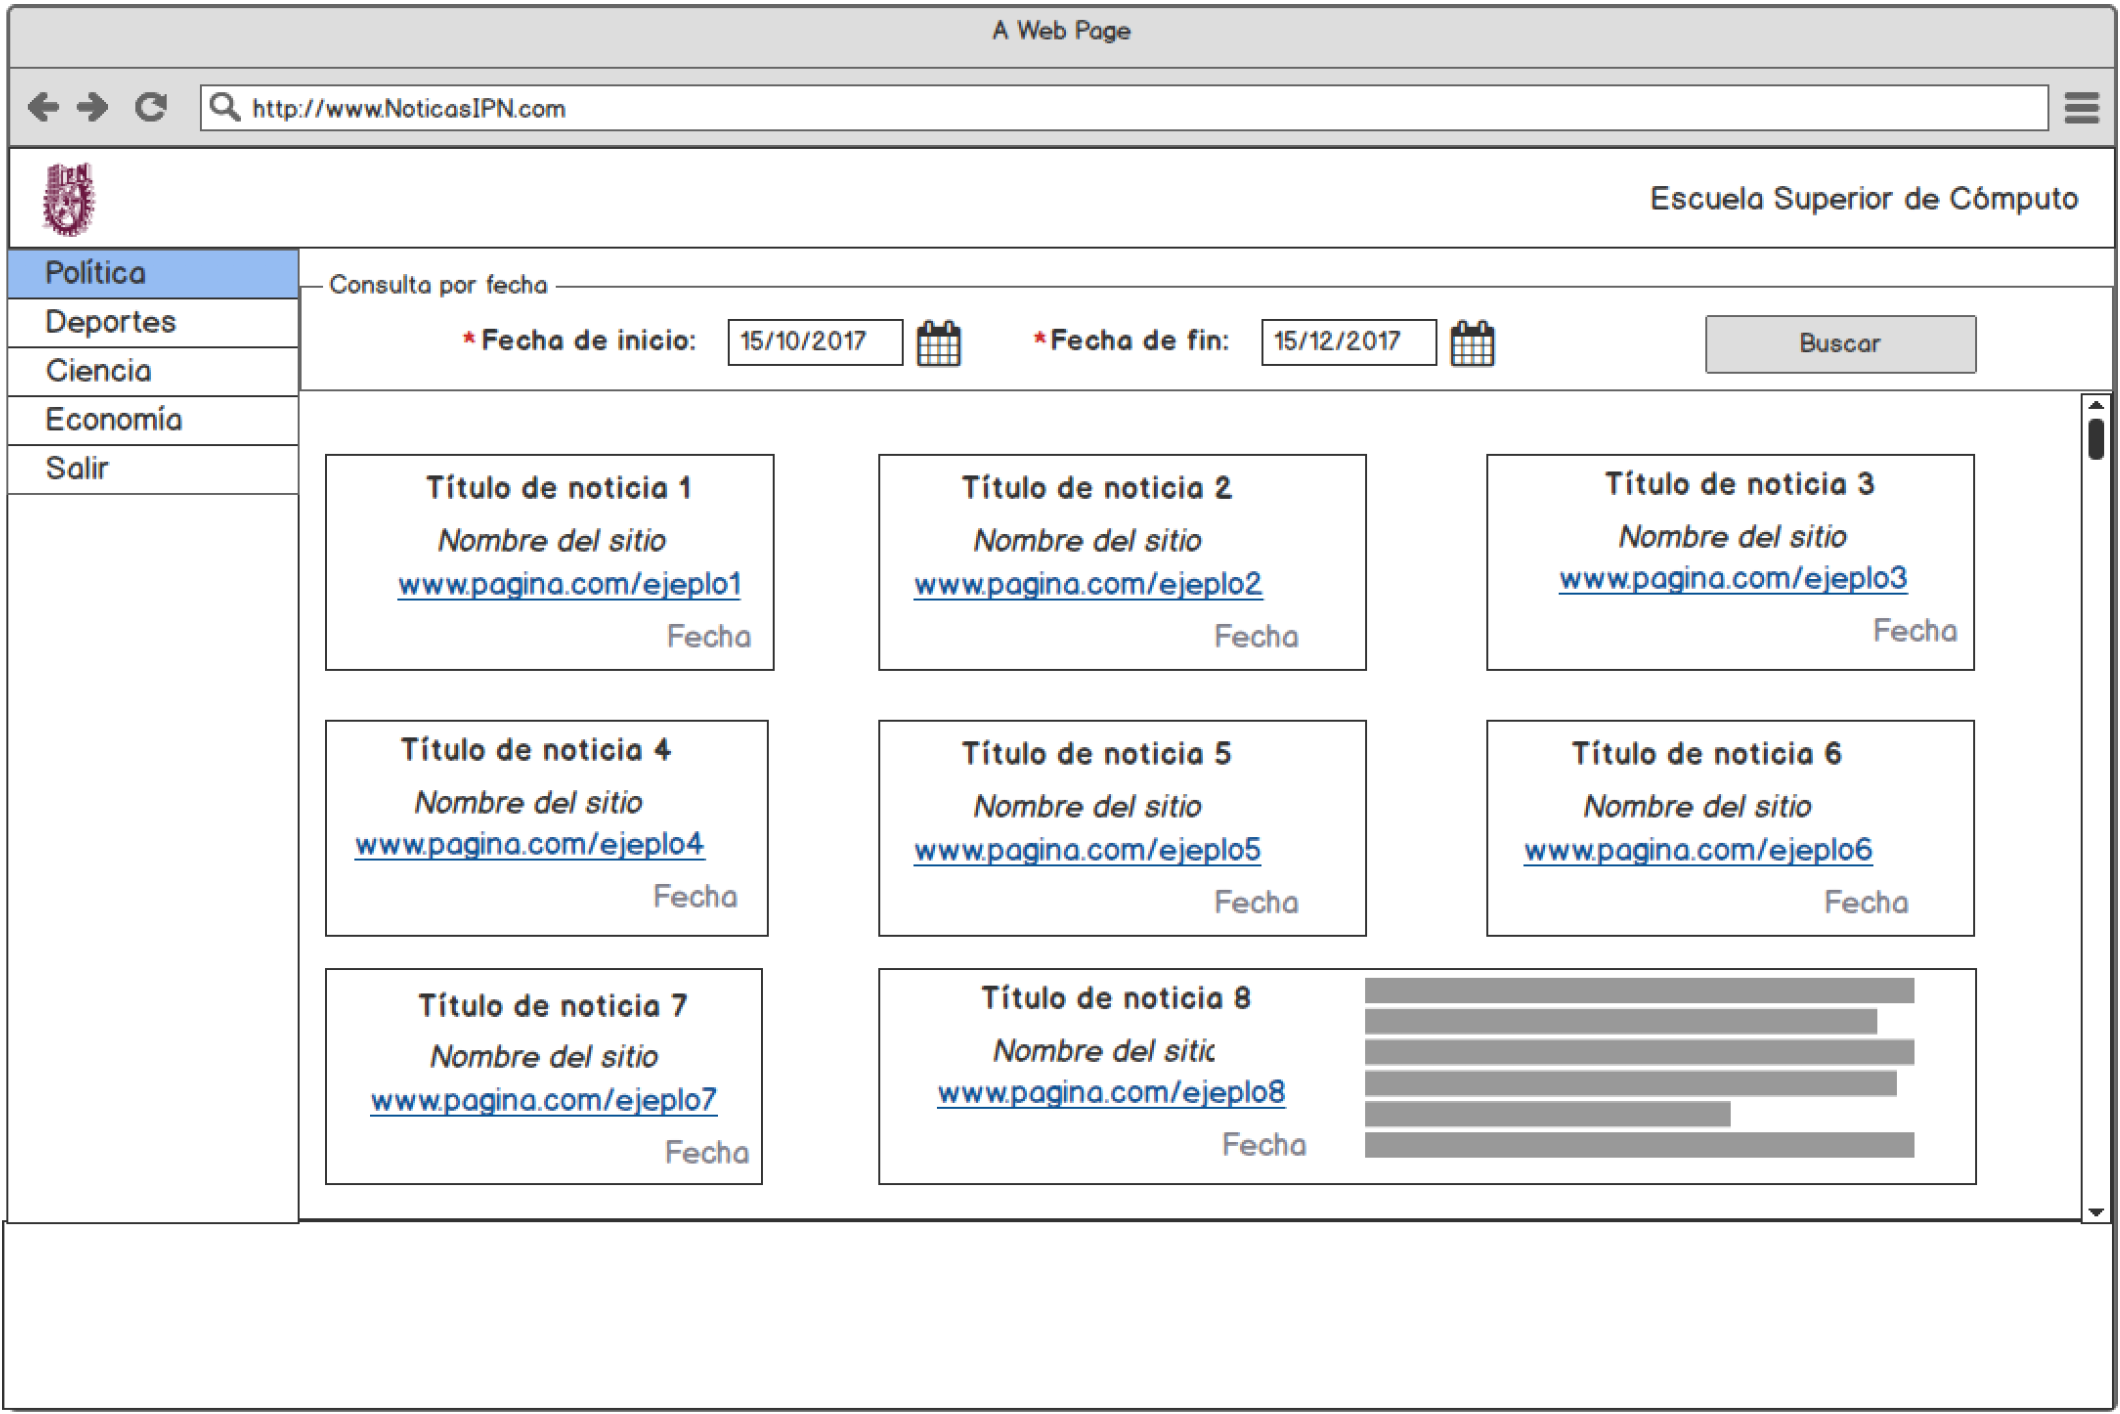
\includegraphics[scale=.3]{imagenes/Pantallas/UI3}
  \caption{Pantalla IU3-Busqueda por fecha}
  \label{fig:IU3}
\end{figure}
\newpage
\subsection{UI4-Página ejemplo}

\Large{\textbf{Objetivo}}\\\\
\normalsize{Texto}\\



\Large{\textbf{Descripción}}\\
\normalsize{Texto}\\


\Large{\textbf{Comandos}}\\
\normalsize{Texto}

\begin{itemize}
	\item Lorem ipsum
	\item Lorem ipsum
	\item Lorem ipsum
\end{itemize}

\Large{\textbf{Referencia}}\\\\
\normalsize{Nombre Caso de uso}

\begin{figure}
  \centering
	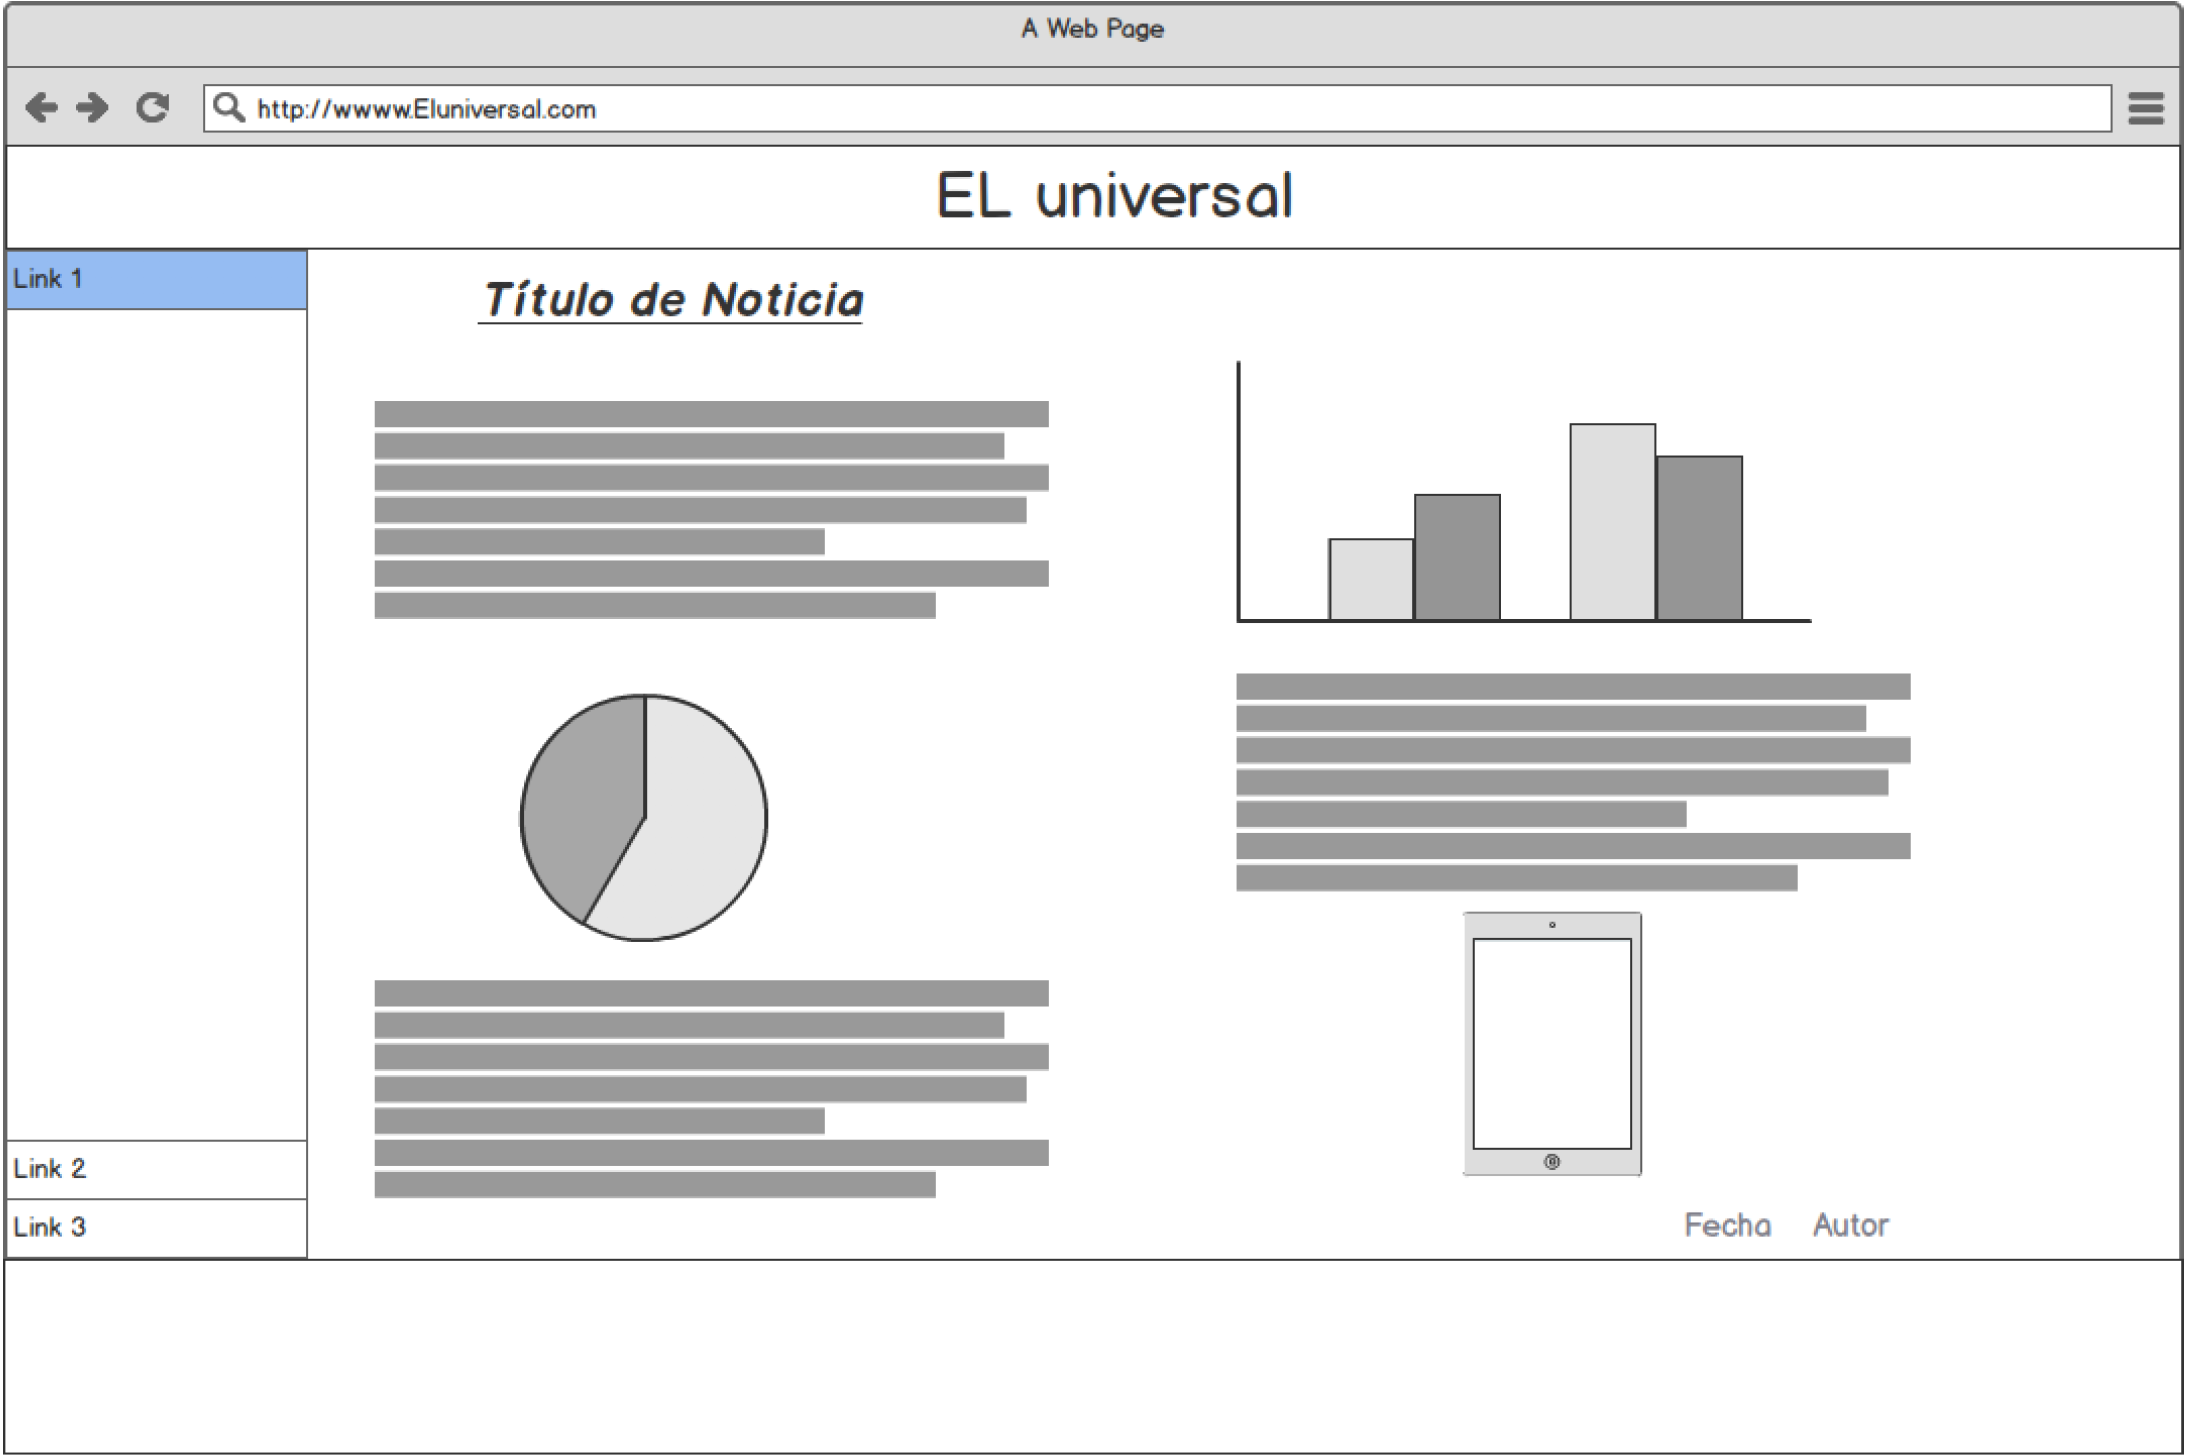
\includegraphics[scale=.3]{imagenes/Pantallas/UI4}
  \caption{Pantalla IU4-Página ejemplo}
  \label{fig:IU4}
\end{figure}
\newpage




